% Panel (d): coupling between the irradiation/segregation and oxidation paths.
% Read left to right: irradiation on the far left, oxide layer on the far right.
% Column widths are set from measured label widths, so no label is forced to break:
%   "Lattice velocity" 2.02 cm and $v_lat = v_lat^RIS + v_ox$ 2.25 cm set column 2.
\documentclass[12pt,border=2pt,tikz]{standalone}

\usepackage{amsmath}

\newcommand{\GB}{\mathrm{GB}}
\newcommand{\eff}{\mathrm{eff}}
\newcommand{\lat}{\mathrm{lat}}
\newcommand{\ox}{\mathrm{ox}}
\newcommand{\Ox}{\mathrm{O}}

\usetikzlibrary{arrows.meta}

\definecolor{cEdge}{RGB}{40,40,44}
\definecolor{cAcc}{RGB}{20,72,124}      % oxidation path (as in a, c)
\definecolor{cAccBg}{RGB}{228,238,247}
\definecolor{cRIS}{RGB}{24,104,66}      % irradiation / segregation path (as in a)
\definecolor{cRISBg}{RGB}{231,243,236}

\hyphenpenalty=10000 \exhyphenpenalty=10000

\begin{document}
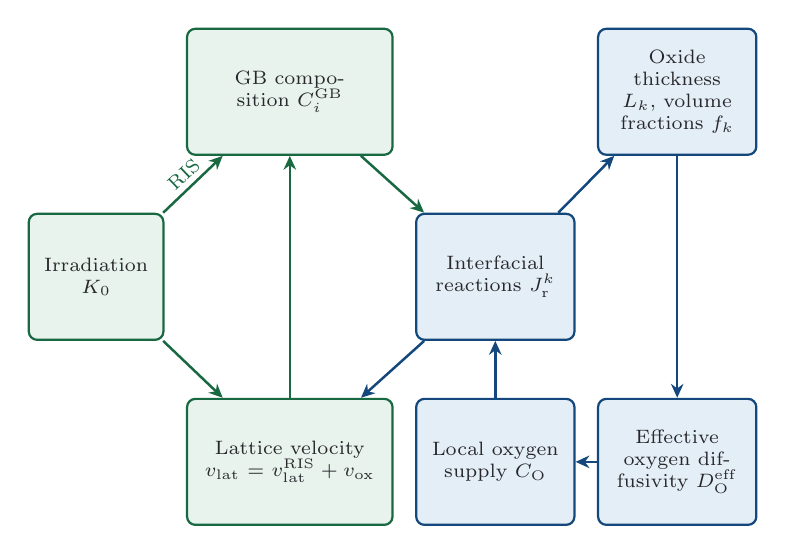
\begin{tikzpicture}[
  x=1cm,y=1cm, font=\scriptsize, color=cEdge,
  box/.style={rounded corners=3pt, draw, line width=0.8pt,
              align=center, minimum height=1.60cm, inner sep=0.13cm, text=cEdge},
  ris/.style ={box, draw=cRIS, fill=cRISBg},
  oxi/.style ={box, draw=cAcc, fill=cAccBg},
  wA/.style  ={text width=1.45cm},
  wB/.style  ={text width=2.35cm},
  wC/.style  ={text width=1.75cm},
  aris/.style={-{Stealth[length=5pt,width=4.5pt]}, line width=0.9pt, draw=cRIS},
  aoxi/.style={-{Stealth[length=5pt,width=4.5pt]}, line width=0.9pt, draw=cAcc},
]

% columns: 0.855 (w 1.71) / 3.315 (w 2.61) / 5.925 (w 2.01) / 8.235 (w 2.01)
% rows:    5.35 / 3.00 / 0.65
\node[ris,wA] (irr)  at (0.855,3.00) {Irradiation $K_0$};
\node[ris,wB] (cgb)  at (3.315,5.35) {GB composition $C_i^{\GB}$};
\node[ris,wB] (lat)  at (3.315,0.65) {Lattice velocity
                                      $v_{\lat}=v_{\lat}^{\mathrm{RIS}}+v_{\ox}$};
\node[oxi,wC] (jr)   at (5.925,3.00) {Interfacial reactions $J_{\mathrm{r}}^{k}$};
\node[oxi,wC] (sup)  at (5.925,0.65) {Local oxygen supply $C_{\Ox}$};
\node[oxi,wC] (ox)   at (8.235,5.35) {Oxide thickness $L_k$, volume fractions $f_k$};
\node[oxi,wC] (deff) at (8.235,0.65) {Effective oxygen diffusivity $D_{\Ox}^{\eff}$};

% ----- irradiation drives both the GB chemistry and the lattice ---------
\draw[aris] (irr) -- (cgb) node[midway,above,sloped,inner sep=2pt,cRIS] {RIS};
\draw[aris] (irr) -- (lat);

% ----- forward path, left to right --------------------------------------
\draw[aris] (cgb) -- (jr);
\draw[aoxi] (jr)  -- (ox);

% ----- return path: oxide chemistry sets the oxygen that comes back -----
\draw[aoxi] (ox)   -- (deff);
\draw[aoxi] (deff) -- (sup);
\draw[aoxi] (sup)  -- (jr);

% ----- oxidation feeds back on the metal --------------------------------
\draw[aoxi] (jr)  -- (lat);
\draw[aris] (lat) -- (cgb);

\end{tikzpicture}
\end{document}
